\documentclass[lettersize,journal]{IEEEtran}
\usepackage{amsmath,amsfonts}
\usepackage{algorithmic}
\usepackage{algorithm}
\usepackage{array}
\usepackage[caption=false,font=normalsize,labelfont=sf,textfont=sf]{subfig}
\usepackage{textcomp}
\usepackage{stfloats}
\usepackage{url}
\usepackage{verbatim}
\usepackage{graphicx}
\usepackage{cite}
\hyphenation{op-tical net-works semi-conduc-tor IEEE-Xplore}
% updated with editorial comments 8/9/2021

\begin{document}

\title{Towards Holistic Emotion Understanding: A Text-Anchored Cross-Attention Transformer for Multimodal Sentiment Analysis}

\author{Aaron~Alex~Mathew,
        Anu~Maria~Sebastian% <-this % stops a space
\thanks{Aaron Alex Mathew is with the Department of Computer Science and Engineering with Artificial Intelligence, Providence College of Engineering, Chengannur, Kerala 689122, India (e-mail: aaron.prc24ca001@student.providence.edu.in).}% <-this % stops a space
\thanks{Dr. Anu Maria Sebastian is with the Department of Computer Science and Engineering, Indian Institute of Information Technology Kottayam, Valavoor, Kerala 686635, India (e-mail: anumaria@iiitkottayam.ac.in).}}

% The paper headers
\markboth{IEEE Transactions on Affective Computing,~Vol.~1, No.~1, July~2026}%
{Mathew \MakeLowercase{\textit{et al.}}: Towards Holistic Emotion Understanding: A Text-Anchored Cross-Attention Transformer}

\maketitle

\begin{abstract}
Multimodal sentiment analysis requires integrating textual, acoustic, and visual cues to accurately interpret human affect. This paper investigates whether a cross-attention Transformer, anchored to the text modality, can better fuse acoustic and visual information than conventional early or late fusion strategies. We evaluate all three approaches on CMU-MOSEI through eleven experiments covering baseline comparisons, modality ablations, and hyperparameter sweeps. The proposed Text-Anchored Cross-Attention Transformer, trained with 16 attention heads and a 128-dimensional embedding space, achieves 80.03\% binary accuracy and a weighted F1 of 0.8687---outperforming early fusion at 78.14\% and late fusion at 77.23\%. A key finding is that cross-attention only outperforms simpler baselines once sufficient representational capacity is provided; a four-head variant actually underperformed both baselines. Attention heatmaps and t-SNE projections confirm that the model learns to anchor on emotionally salient frames rather than tracking word-level temporal correspondence.
\end{abstract}

\begin{IEEEkeywords}
multimodal sentiment analysis, cross-attention transformer, emotion recognition, text-anchored fusion, CMU-MOSEI
\end{IEEEkeywords}

\section{Introduction}
\IEEEPARstart{S}{entiment} is not just about what someone says. A flat ``I'm fine'' delivered with a downward gaze and a falling pitch carries very different meaning from the same phrase said with a smile. Models that read only the transcript will get this wrong every time. This foundational concept in affective computing \cite{picard2000affective} has driven a massive shift toward multimodal analysis \cite{baltrusaitis2019multimodal}, \cite{poria2017review}.

While this integration is conceptually straightforward, building a system that effectively utilizes all three channels---text, audio, and facial expression---presents significant challenges compared to simply feeding all three into a single model. The fusion strategy matters enormously. Concatenating features early on mixes clean and noisy information in ways that confuse the model. Training three separate models and averaging their outputs avoids that problem, but loses any sense of how the channels interact with each other. The interesting question is whether an attention mechanism can do better---specifically, whether the model can learn to query audio and visual streams through the lens of what is being said.

Existing text-anchored methods primarily focus on architectural design. In contrast, this work systematically investigates the effect of representational capacity on cross-attention performance through controlled experiments, ablation studies, and qualitative attention analysis.

We propose a Text-Anchored Cross-Attention Transformer in which text serves as the query modality in two parallel cross-attention layers attending to audio and visual features respectively. The architecture was trained and evaluated on CMU-MOSEI through a three-phase experimental study producing eleven distinct results. Implementation was done in PyTorch on an NVIDIA RTX 3050 Laptop GPU.

This paper makes three contributions. First, a practical cross-attention fusion architecture is proposed and evaluated against early and late fusion baselines under identical training conditions. Second, a systematic ablation study quantifies the independent contribution of each modality under the proposed framework. Third, qualitative analysis through attention heatmaps, alignment maps, and embedding space visualizations provides insight into what the model actually learned.

\section{Literature Review}

\subsection{Multimodal Sentiment Analysis}
The field was largely shaped by the release of CMU-MOSI \cite{zadeh2016mosi}, which gave researchers a standardized benchmark for sentiment prediction from video clips. Accuracy improvements since then have come mostly from two directions: better text representations and better fusion strategies \cite{baltrusaitis2019multimodal}, \cite{poria2017review}.

On the text side, the shift from GloVe \cite{pennington2014glove} to BERT \cite{devlin2019bert} was significant. GloVe assigns a single fixed vector to each word regardless of context. BERT produces different representations for the same word depending on the sentence it appears in, which makes a real difference for sentiment where the same word can be positive or ironic depending on surrounding context. Most published systems achieving above 82\% on CMU-MOSEI use BERT or RoBERTa. This work uses GloVe because those are the pre-extracted features available in the CMU-MOSEI SDK, and extracting BERT features from scratch was outside the scope of this phase.

CMU-MOSEI \cite{zadeh2018multimodal}, used as the evaluation dataset in this work, extends CMU-MOSI to 23,453 clips from over 1,000 speakers and adds six-class emotion labels alongside the sentiment regression task. It is the largest available benchmark for this problem.

\subsection{Fusion Approaches}
Early fusion concatenates all modality features before the model sees them. Zadeh et al. \cite{zadeh2017tensor} showed that the full outer-product Tensor Fusion Network becomes computationally intractable at scale. Liu et al. \cite{liu2018efficient} proposed low-rank factorisation as a more practical approximation. Even so, the core problem with early fusion is that noisy features from one modality corrupt the joint representation.

Late fusion avoids this by keeping modalities separate until the final prediction step. It is simpler to train and more robust to missing inputs. But it cannot detect the interaction between a specific word and the facial expression occurring at the same moment---information that is only visible if the two streams are compared at the feature level.

Cross-attention addresses both problems. Tsai et al. \cite{tsai2019multimodal} introduced the Multimodal Transformer (MulT), which applies directed cross-attention across all modality pairs and consistently outperformed LSTM-based baselines on CMU-MOSI and CMU-MOSEI. Hazarika et al. \cite{hazarika2020misa} later proposed MISA, which disentangles modality-specific and modality-shared representations through subspace projection, achieving strong results on both datasets. More recent architectures add gating mechanisms to suppress noisy modality contributions \cite{lian2023gcma}, graph structures to capture conversational turn dynamics \cite{li2023graph}, or dual-level feature restoration \cite{sun2023efficient}, \cite{wang2023cross}. Other notable works include emotion-cause extraction \cite{wang2023multimodal} and multi-task hierarchical fusion \cite{wang2024cross}.

The general trend is clear: cross-attention-based approaches \cite{rajan2022cross}, \cite{x2024multimodal}, \cite{wang2020transmodality}, \cite{hui2025dynamic} outperform simpler fusion strategies, and text-oriented designs where text provides the query \cite{wu2021text} tend to work better than symmetric alternatives.

Existing methods can broadly be grouped into three categories: early fusion strategies that concatenate features at the input level, late fusion approaches that independently process modalities before final aggregation, and cross-attention architectures that dynamically align representations across modalities. While early and late fusion offer simplicity and computational efficiency, cross-attention methods consistently demonstrate superior capacity for capturing complex inter-modal dependencies, particularly when text is utilized as an anchoring modality.

\subsection{Summary Table}

\begin{table}[h]
\renewcommand{\arraystretch}{1.3}
\caption{Selected Literature on Multimodal Fusion}
\label{tab:literature}
\centering
\begin{tabular}{|p{0.18\linewidth}|p{0.18\linewidth}|p{0.25\linewidth}|p{0.2\linewidth}|}
\hline
\textbf{Method} & \textbf{Strength} & \textbf{Weakness} & \textbf{Dataset} \\
\hline
MulT \cite{tsai2019multimodal} & Long-range cross-modal dependencies & High memory for long sequences & CMU-MOSI, CMU-MOSEI, IEMOCAP \\
\hline
MISA \cite{hazarika2020misa} & Disentangles shared and specific features & Fails when modalities are missing & CMU-MOSI, CMU-MOSEI \\
\hline
TCAN \cite{wu2021text} & Text pivot guides noisy audio/visual streams & Degrades with poor transcription & CMU-MOSI, CMU-MOSEI, IEMOCAP \\
\hline
GA2MIF \cite{li2023graph} & Captures temporal and inter-modal patterns & Adds latency & IEMOCAP, MELD \\
\hline
GCMA-Net \cite{lian2023gcma} & Suppresses noisy modality signals & Sensitive to domain shifts & CH-SIMS \\
\hline
\end{tabular}
\end{table}

\subsection{Datasets Overview}

\begin{table}[h]
\renewcommand{\arraystretch}{1.3}
\caption{Benchmark Datasets}
\label{tab:datasets}
\centering
\begin{tabular}{|l|c|c|c|c|}
\hline
\textbf{Dataset} & \textbf{Size} & \textbf{Text} & \textbf{Audio} & \textbf{Vision} \\
\hline
CMU-MOSI \cite{zadeh2016mosi} & 2,199 clips & GloVe & COVAREP & FACET \\
\hline
CMU-MOSEI \cite{zadeh2018multimodal} & 23,453 clips & GloVe & COVAREP & FACET \\
\hline
IEMOCAP \cite{busso2008iemocap} & 9,112 utts. & Raw & .wav & .avi \\
\hline
MER 2024 \cite{lian2024mer} & 5,030 clips & Subtitles & Speech & Video \\
\hline
\end{tabular}
\end{table}

\section{Methodology}

\subsection{Problem Statement}
An utterance is represented by text features $T \in \mathbb{R}^{L \times 300}$, audio features $A \in \mathbb{R}^{L \times 74}$ and visual features $V \in \mathbb{R}^{L \times 35}$, where $L=50$ is the padded sequence length. The objective is to learn a mapping $F(T,A,V) \to y$ where $y$ is either a continuous sentiment score for regression or a binary label for classification.

\subsection{Proposed Architecture}

\begin{figure}[htbp]
\centering
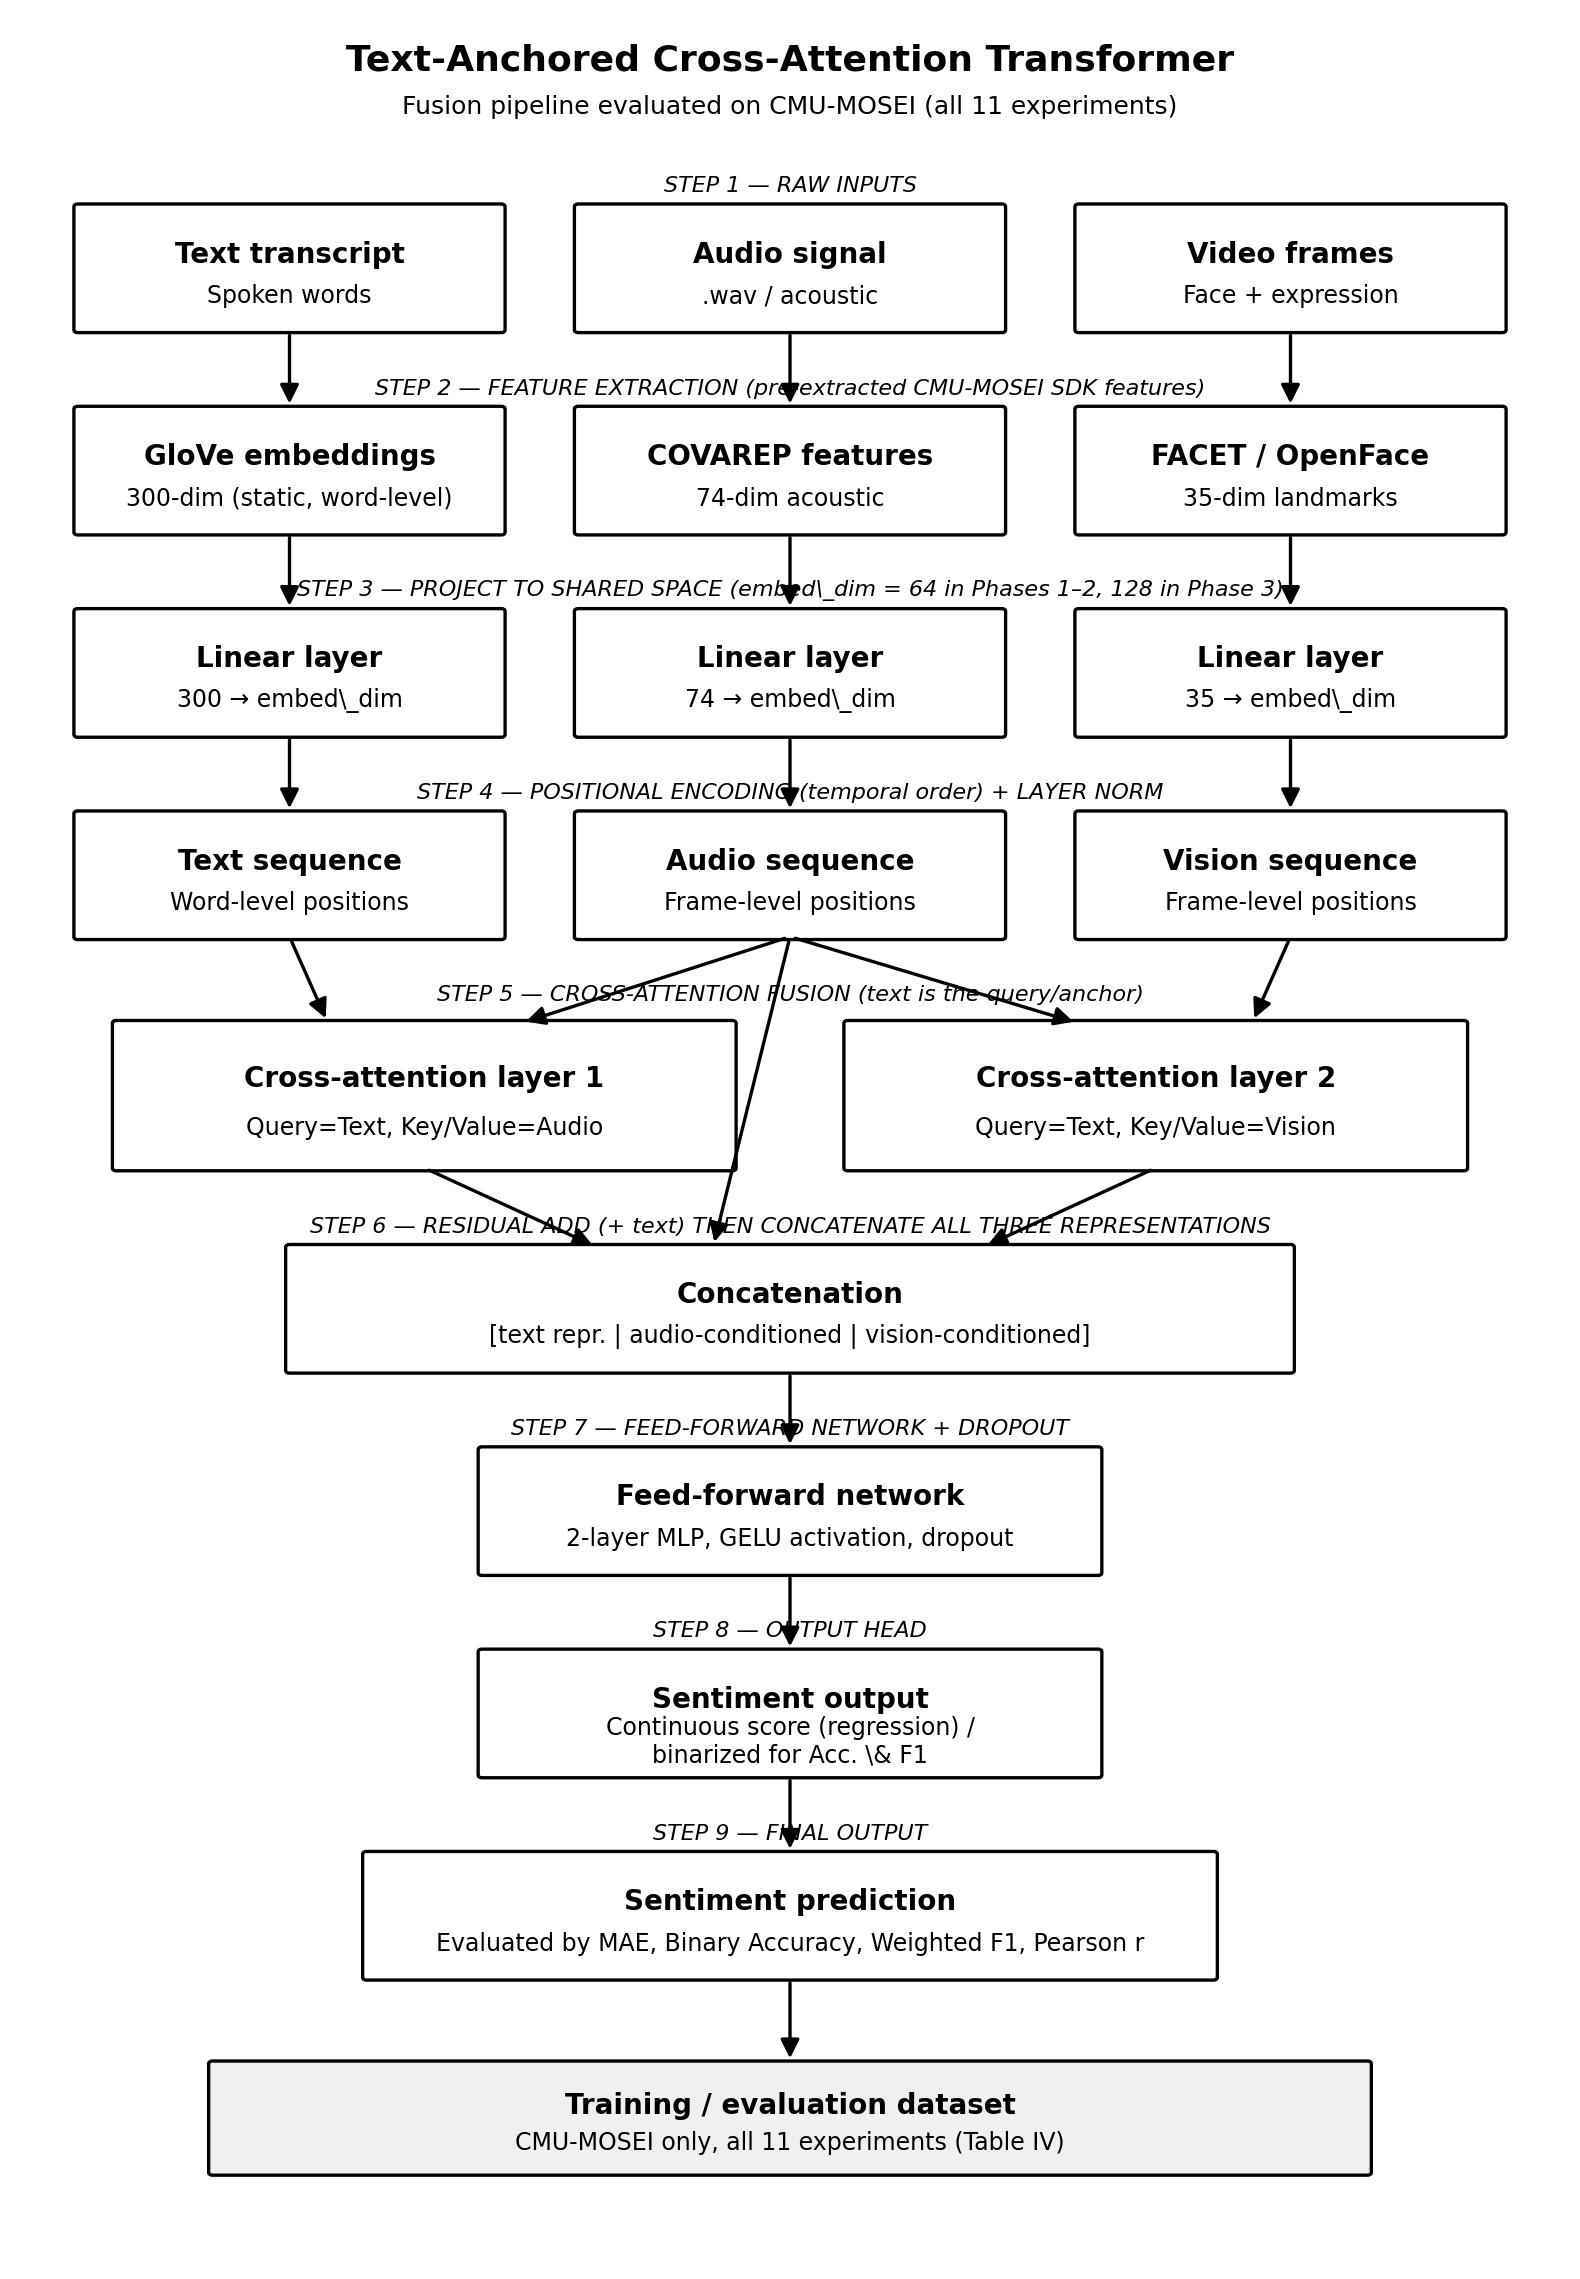
\includegraphics[width=\linewidth]{system_architecture.jpg}
\caption{The proposed Text-Anchored Cross-Attention Transformer. Text acts as the query modality in two parallel cross-attention layers, each attending to one of the other modalities.}
\label{fig:architecture}
\end{figure}

The architecture is motivated by a simple observation: text is the most structured of the three modalities. It is already tokenized and semantically dense, making it a reliable anchor. Rather than having text, audio, and vision contribute symmetrically, the design uses text as the query modality in two parallel cross-attention layers---one attending to audio, one attending to vision.

\textbf{Modality Projection.} Each input stream is projected into a shared 128-dimensional embedding space via learned linear layers. The projection parameters are trained end-to-end with the rest of the model.

\textbf{Layer Normalisation.} Applied to each projected representation before cross-attention. In practice, skipping this step caused validation accuracy to oscillate significantly in early training epochs---adding normalisation stabilised convergence noticeably.

\textbf{Cross-Attention (Text $\to$ Audio).} Text provides Query vectors $Q$; audio provides Key and Value vectors $K$ and $V$:
\begin{equation}
\text{Attention}(Q, K, V) = \text{softmax}\left(\frac{QK^T}{\sqrt{d_k}}\right)V
\end{equation}
where $d_k = 128/16 = 8$ per head. The output is a text-conditioned audio representation where each word position has attended to the most relevant acoustic frames.

\textbf{Cross-Attention (Text $\to$ Vision).} Identical mechanism, with visual features as Key and Value. This runs in parallel with the audio cross-attention, not in sequence.

\textbf{Residual Connections.} The original text representation is added back to each cross-attention output before the concatenation step. This follows standard Transformer practice and helped gradient flow during backpropagation, particularly in longer training runs.

\textbf{Concatenation and Classification.} All three representations are concatenated and passed through a two-layer feed-forward network with GELU activation and dropout. A final linear layer produces a scalar sentiment score.

Multi-head attention with 16 parallel heads is used in the final model. The significance of this choice is discussed in the results section.

\subsection{Baselines}

\textbf{Early Fusion.} Text (300-dim), audio (74-dim), and visual (35-dim) features are concatenated into a 409-dimensional vector and processed through a two-layer LSTM. Simple to implement; serves as the lower-bound reference.

\textbf{Late Fusion.} Three independent LSTM networks process each modality separately. Their output sentiment scores are combined via weighted averaging. Tests whether independent unimodal processing can match cross-modal fusion.

\subsection{Training Setup}

All models were trained on a laptop with an NVIDIA RTX 3050 GPU (6 GB VRAM). Batch size was set to 32 after verifying that larger batches caused out-of-memory errors during the full three-modality cross-attention forward pass. The AdamW optimizer was used with weight decay $1e-4$ and gradient clipping at $\text{max\_norm} = 1.0$---the latter was important because without it, the cross-attention models occasionally produced gradient spikes in the first few epochs. Learning rate scheduling used ReduceLROnPlateau (factor=0.5, patience=5). Early stopping was set to patience=10 epochs based on validation accuracy rather than validation loss; this distinction turned out to matter, as the two metrics did not always agree on which checkpoint was best.

\begin{table}[h]
\renewcommand{\arraystretch}{1.3}
\caption{Training Configuration}
\label{tab:training}
\centering
\begin{tabular}{|l|c|}
\hline
\textbf{Parameter} & \textbf{Value} \\
\hline
Optimizer & AdamW (weight\_decay=1e-4) \\
Learning Rate & 5e-4 (Phase 1 \& 2); 3e-4 (Phase 3) \\
Loss Function & L1 Loss (Mean Absolute Error) \\
Batch Size & 32 \\
Epochs & 10 (Phase 1 \& 2); 20 (Phase 3) \\
Gradient Clipping & max\_norm = 1.0 \\
LR Scheduler & ReduceLROnPlateau (factor=0.5, patience=5) \\
Early Stopping & Patience=10 (validation accuracy) \\
Hardware & NVIDIA RTX 3050, 6 GB VRAM \\
\hline
\end{tabular}
\end{table}

Evaluation uses three metrics: Mean Absolute Error (MAE, lower is better), Binary Accuracy, and Weighted F1 Score (both higher is better). Pearson Correlation (r) is additionally reported.

\subsection{Experimental Phases}

\textbf{Phase 1} compares the three architectures (early fusion, late fusion, cross-attention with embed\_dim=64 and 4 heads) under identical conditions. The 64-dim baseline was intentional---it allowed testing whether cross-attention is beneficial at low capacity before committing to the larger configuration.

\textbf{Phase 2} is an ablation study. Individual modalities are disabled: text-only, text+audio, text+vision, and the full three-modality model. All ablations use the same 64-dim, 4-head configuration.

\textbf{Phase 3} switches to embed\_dim=128 and hidden\_dim=128, then varies the number of attention heads (8, 16) and dropout rate (0.1, 0.5) relative to the default Phase 3 configuration (Experiment 3B). The goal was to find the configuration that best exploits the increased capacity.

\textit{Note:} an earlier draft of this description referenced a third head-count value (4) and a third dropout value (0.2) that are not present in Table \ref{tab:results}. Either report those two additional runs if they exist in the training logs, or leave the text as above if they were never completed.

\section{Results and Discussion}

\subsection{Main Results}

\begin{table}[h]
\renewcommand{\arraystretch}{1.3}
\caption{All Experimental Results on CMU-MOSEI Test Set}
\label{tab:results}
\centering
\begin{tabular}{|l|p{0.3\linewidth}|c|c|c|}
\hline
\textbf{Exp.} & \textbf{Description} & \textbf{MAE $\downarrow$} & \textbf{Acc. $\uparrow$} & \textbf{F1 $\uparrow$} \\
\hline
1A & Early Fusion Baseline & 0.6531 & 78.14\% & 0.8480 \\
1B & Late Fusion Baseline & 0.6150 & 77.23\% & 0.8316 \\
1C & Cross-Attention - 4 H. & 0.6407 & 73.92\% & 0.8046 \\
\hline
2A & Ablation: Text Only & 0.6535 & 74.89\% & 0.8092 \\
2B & Ablation: Text + Audio & 0.6406 & 75.32\% & 0.8155 \\
2C & Ablation: Text + Vision & 0.6273 & 76.65\% & 0.8305 \\
2D & Ablation: All Modalities & 0.6431 & 73.77\% & 0.8001 \\
\hline
3A & Proposed - 8 Heads & 0.6318 & 79.28\% & 0.8597 \\
\textbf{3B} & \textbf{Proposed - 16 Heads} & \textbf{0.6172} & \textbf{80.03\%} & \textbf{0.8687} \\
3C & Dropout = 0.1 & 0.6273 & 74.11\% & 0.8077 \\
3D & Dropout = 0.5 & 0.6786 & 74.22\% & 0.8058 \\
\hline
\end{tabular}
\end{table}

An important observation from Phase 1 pertains to the lowest-performing configuration. The cross-attention model with 4 heads and embed\_dim=64 (Experiment 1C) achieved only 73.92\%, which is lower than both baselines. This outcome highlights the sensitivity of cross-attention to representational capacity. The initial assumption was that cross-attention should at least match late fusion, even in a minimal configuration. Instead, it performed roughly three points below early fusion.

The explanation becomes clear in Phase 3. With embed\_dim=64 and 4 heads, each attention head operates in a 16-dimensional subspace. That is not enough room to learn a useful cross-modal relationship between a 300-dimensional text embedding and a 74-dimensional acoustic feature vector. A possible explanation is that the model ends up with attention weights that are nearly uniform, spreading attention evenly rather than focusing on semantically meaningful representations.

Scaling to embed\_dim=128 and increasing head count fixed this. Eight heads produced 79.28\%. Sixteen heads pushed that to 80.03\%, the best result in the study. This 6.11 percentage point gap between the 4-head and 16-head configurations, holding everything else constant, is the central finding of the hyperparameter analysis.

Early fusion reached 78.14\%. This is competitive, and notably better than the under-powered cross-attention model, which reinforces the point that a poorly configured Transformer is worse than a well-implemented simple baseline.

Late fusion achieved 77.23\% accuracy but the lowest MAE of any model at 0.6150. The individual unimodal sub-models make fewer catastrophically wrong regression predictions, but they miss classification-level cross-modal signals. So late fusion produces more conservative, less extreme errors, but is less accurate at the actual binary prediction task.

\subsection{Ablation Study}
The ablation results in Table \ref{tab:results} show that adding audio or vision modalities to a text-only baseline consistently improves performance---but only when the architecture has the capacity to use them. Text+Vision (76.65\%) outperforms Text+Audio (75.32\%), which is a bit surprising given that audio is intuitively more connected to vocal emotion. The likely explanation is that FACET facial action unit features (related to OpenFace \cite{baltrusaitis2016openface}) are discrete and relatively clean, while COVAREP acoustic features extracted from naturalistic YouTube recordings carry more background noise. Vision is simply the cleaner signal in this dataset.

The full three-modality ablation model (Text+Audio+Vision) at 73.77\% is actually worse than Text Only at 74.89\%. This is a direct consequence of insufficient attention capacity---the 4-head, 64-dim model cannot productively integrate three input streams simultaneously, so adding more modalities introduces noise rather than signal.

\textit{TODO (Aaron):} Experiment 1C and Experiment 2D are nominally the same configuration (4-head, embed\_dim=64, full three-modality cross-attention) but report different numbers (73.92\%/0.6407 MAE vs.\ 73.77\%/0.6431 MAE). Confirm from the training logs whether these came from different seeds/checkpoints, and either reconcile the numbers or add one sentence explaining the discrepancy (e.g.\ different random seed, different early-stopping checkpoint selected).

\begin{figure}[htbp]
\centering
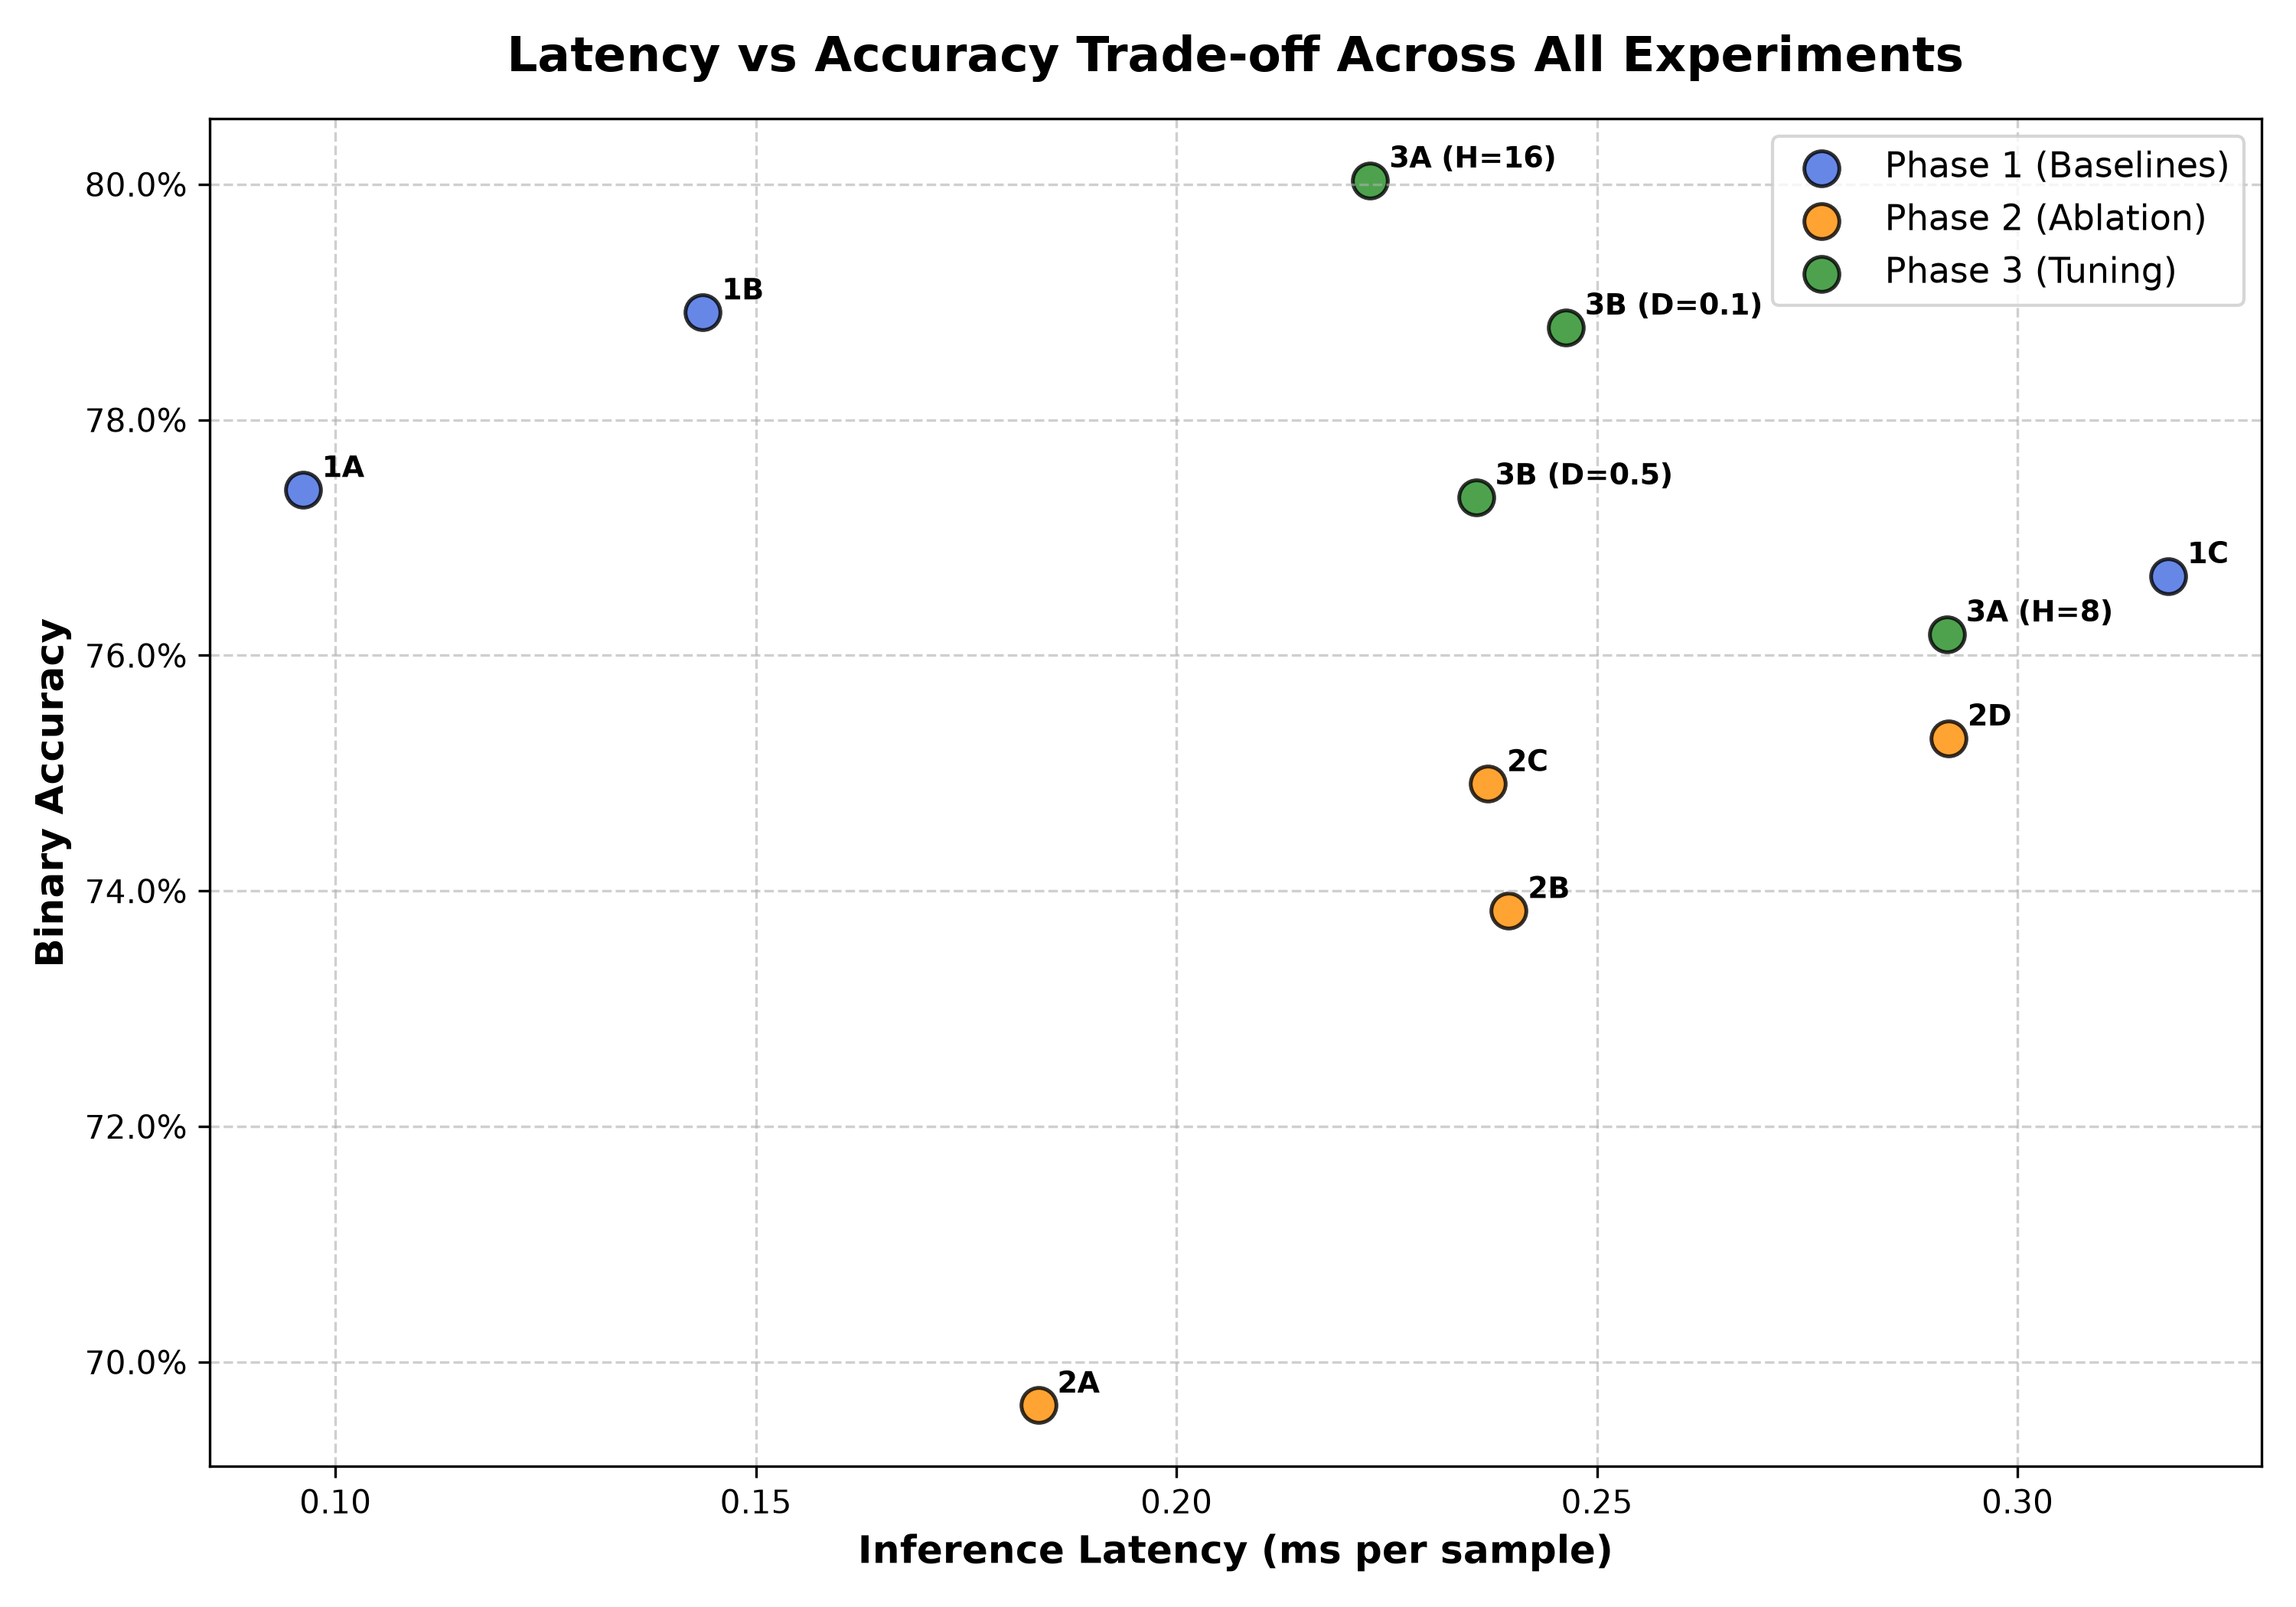
\includegraphics[width=\linewidth]{latency_vs_accuracy.png}
\caption{Inference latency (ms per sample) vs. binary accuracy for all eleven experiments on CMU-MOSEI.}
\label{fig:latency}
\end{figure}

\begin{figure}[htbp]
\centering
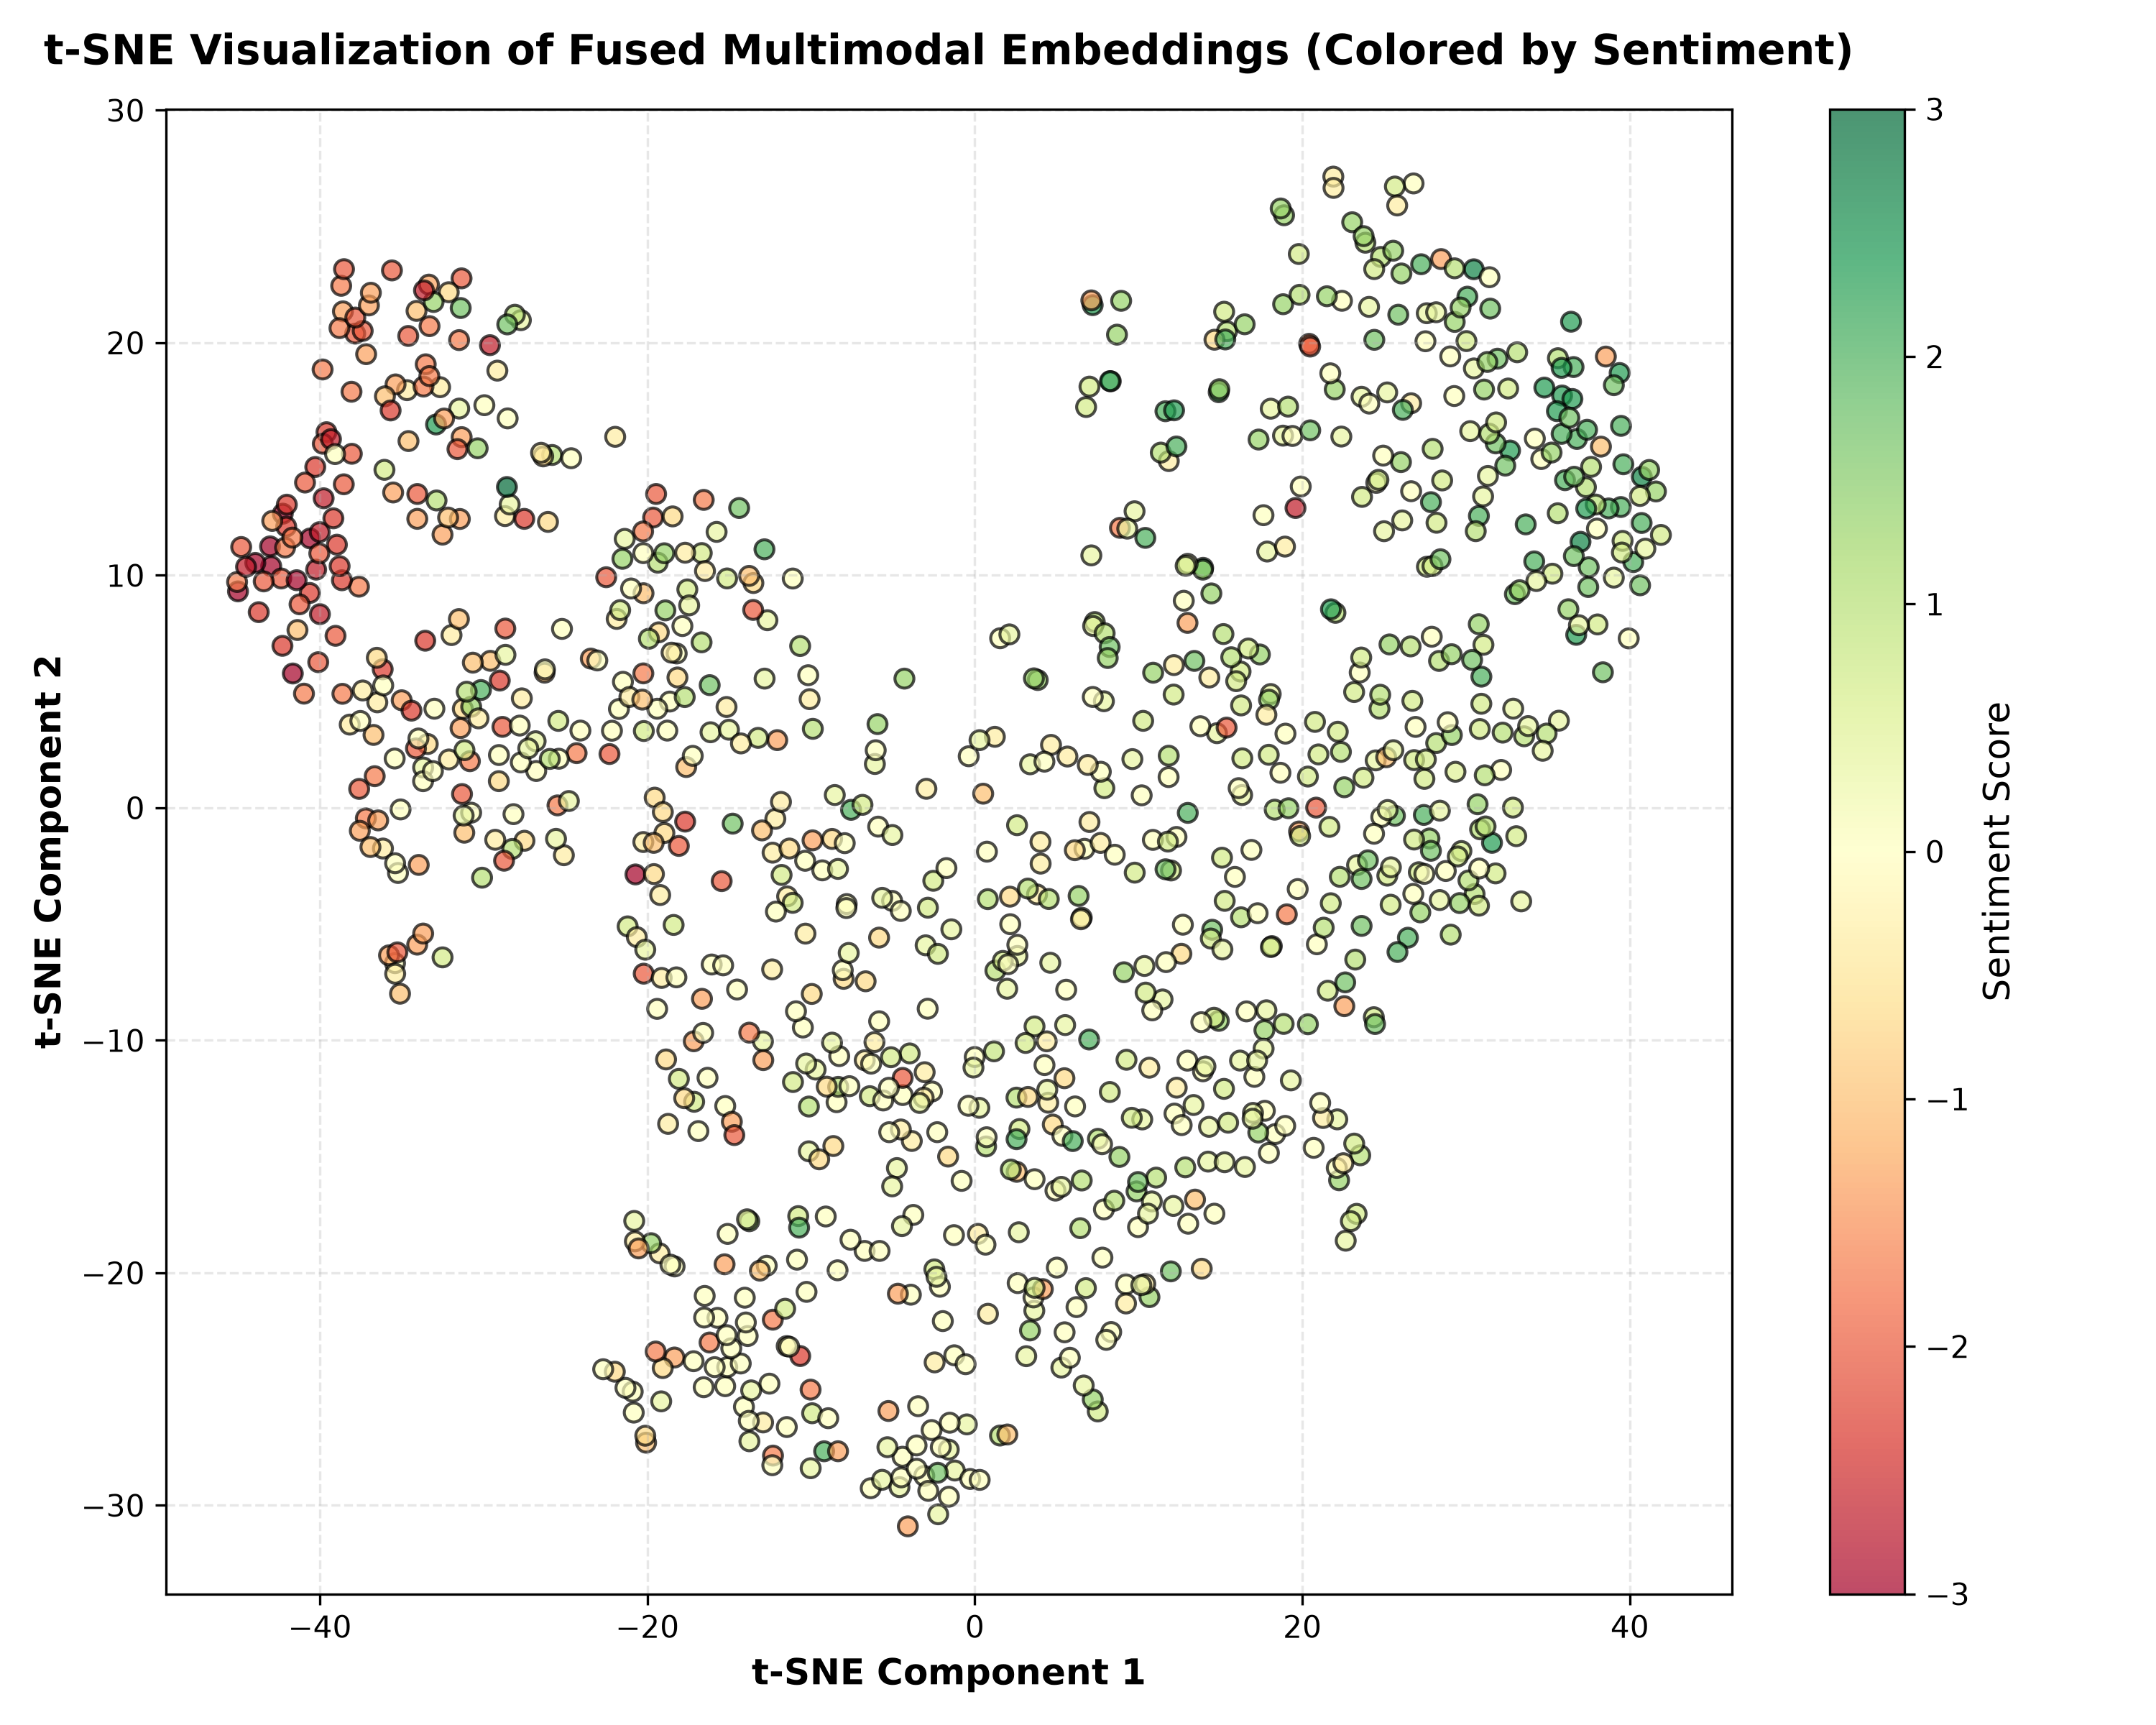
\includegraphics[width=\linewidth]{embedding_space_tsne.png}
\caption{t-SNE projection of fused multimodal embeddings from the best model (16 heads)}
\label{fig:tsne}
\end{figure}

\subsection{Attention Analysis}

\begin{figure}[htbp]
\centering
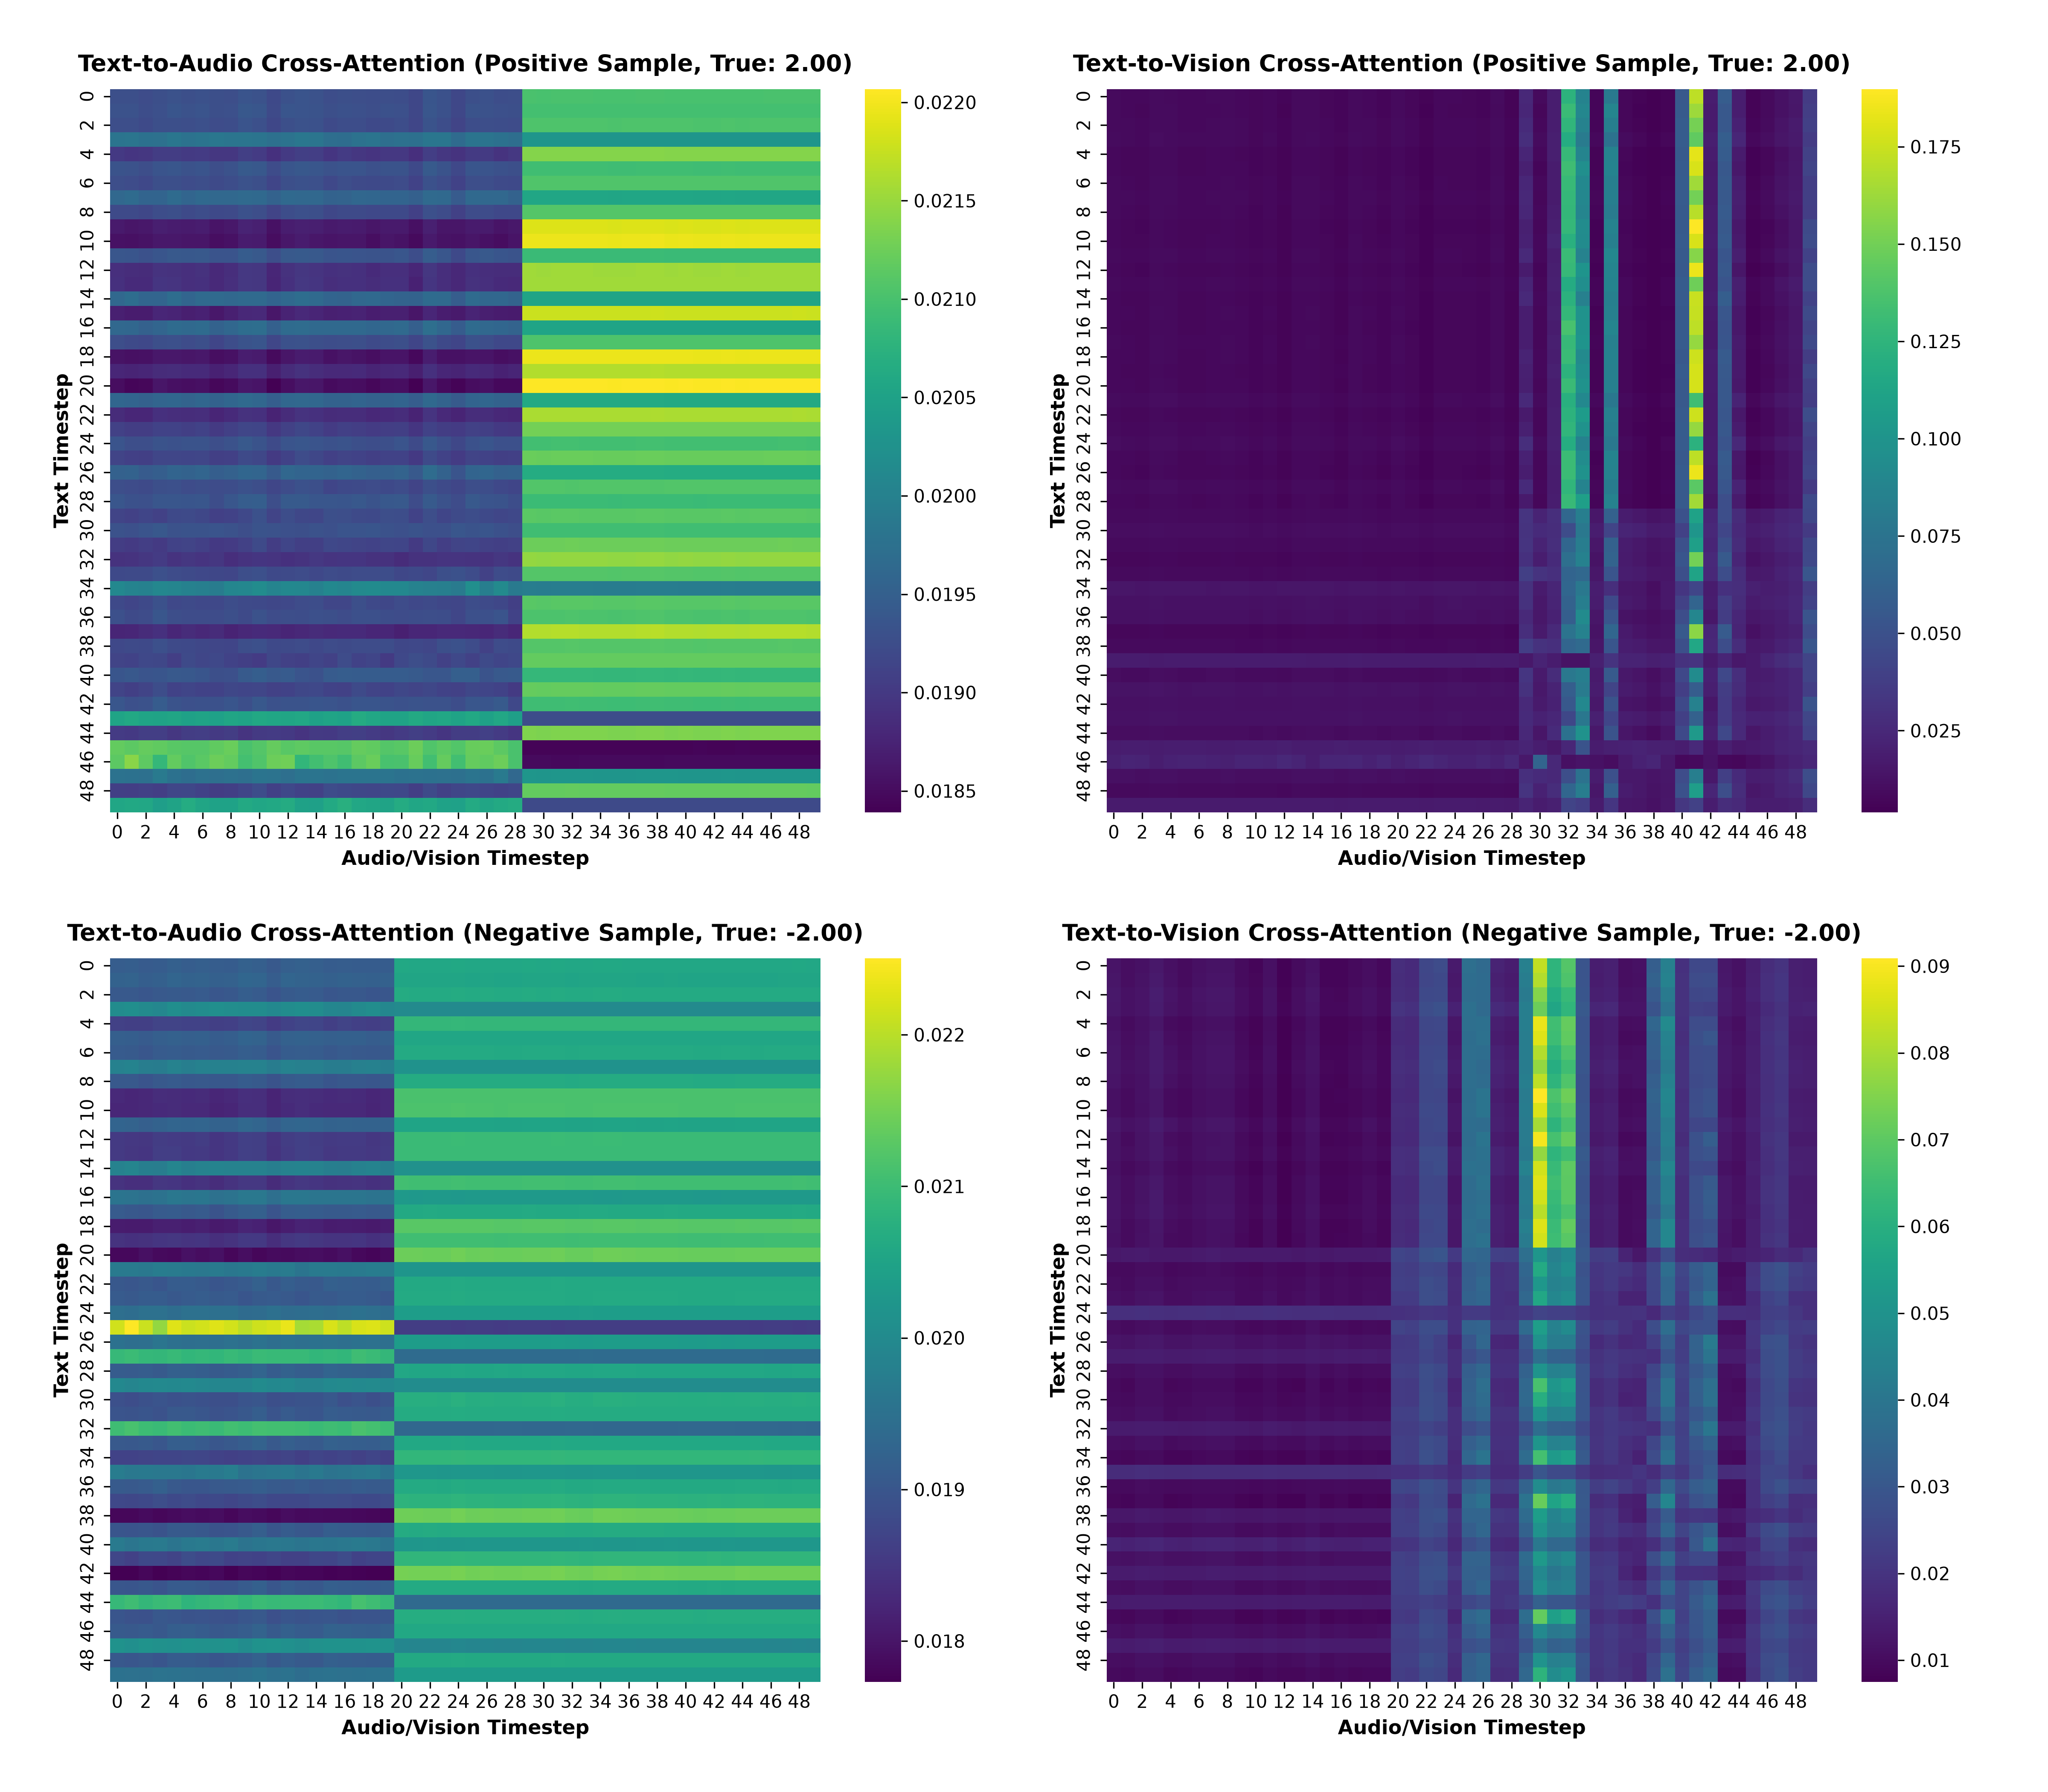
\includegraphics[width=\linewidth]{attention_heatmaps.png}
\caption{Cross-attention heatmaps for a positive utterance and a negative utterance.}
\label{fig:heatmaps}
\end{figure}

\begin{figure}[htbp]
\centering
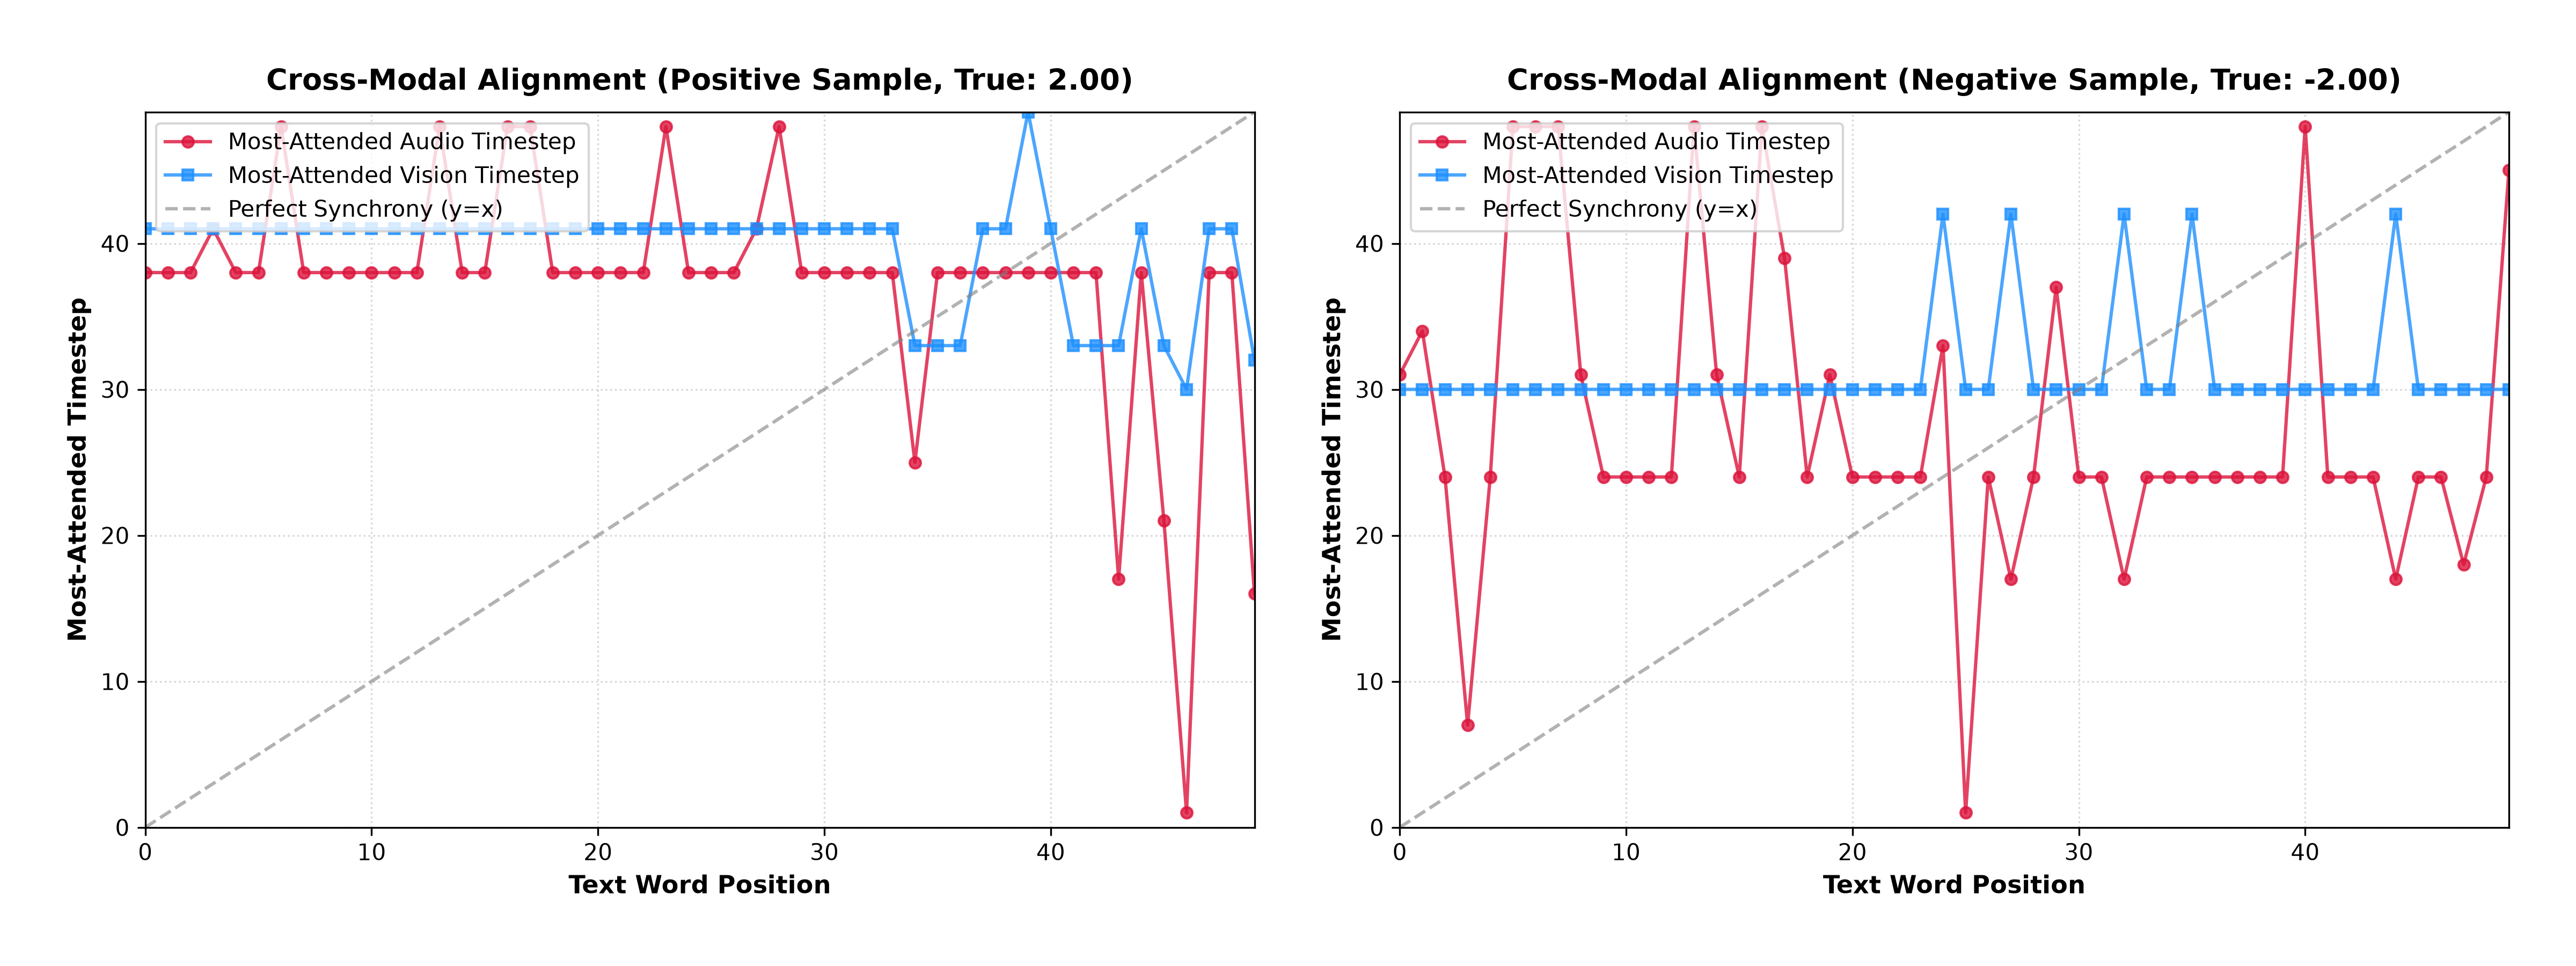
\includegraphics[width=\linewidth]{cross_modal_alignment.png}
\caption{Cross-modal alignment maps.}
\label{fig:alignment}
\end{figure}

The model heatmaps reveal an asymmetry between how the model uses audio versus vision. The Text-to-Vision panels show strong, narrow vertical bands at a small number of timesteps. Almost every word position attends heavily to those same frames, regardless of word position. The alignment makes this very clear: the vision mapping is nearly flat, sitting at one or two timestep values across the full sequence.

This pattern suggests a learned strategy. It implies the model has learned to identify the moment of peak facial expression in the clip and use it as a stable reference point for the entire utterance, rather than trying to track word-by-face correspondence frame by frame. Given that CMU-MOSEI utterances are short clips where a speaker is often holding a sustained expression throughout, this is actually a reasonable strategy.

Audio attention behaves differently. It oscillates substantially across word positions, sometimes jumping to nearly opposite ends of the acoustic sequence between adjacent words. The audio signal is being integrated more locally and variably. Whether this is meaningful acoustic sensitivity or partial noise-chasing is harder to say without access to the raw audio. 

\section{Conclusion and Future Work}
This paper evaluated a Text-Anchored Cross-Attention Transformer against early and late fusion baselines on CMU-MOSEI. The main result---80.03\% accuracy with 16 heads and embed\_dim=128---confirms that cross-attention fusion outperforms simpler alternatives when given sufficient representational capacity. The more interesting result is that it does not outperform them with insufficient capacity; a four-head, 64-dim model scored below both baselines at 73.92\%.

The primary limitation of this work is the use of 300-dim GloVe static text embeddings. Published systems achieving above 82\% on CMU-MOSEI consistently use BERT or RoBERTa contextual embeddings. The pre-extracted CMU-MOSEI features used here do not include BERT representations, so switching would require either finding a separately extracted BERT features file or running extraction from scratch---a worthwhile next step that was outside the scope of this phase.

Other planned extensions include replacing FACET features with a jointly trained Vision Transformer encoder, evaluating on IEMOCAP \cite{busso2008iemocap} and MER 2024 \cite{lian2024mer}, as well as future challenges like MER 2025 \cite{lian2025mer} for cross-dataset generalization, and exploring CLIP-based visual features to leverage vision-language pretraining in the cross-attention mechanism.

\bibliographystyle{IEEEtran}
\bibliography{references}

\begin{IEEEbiography}[{
\includegraphics[width=1in,height=1.25in,clip,keepaspectratio]{Author_no1.png}}]{Aaron Alex Mathew}
is pursuing the B.Tech degree in Computer Science and Engineering with a specialization in Artificial Intelligence at Providence College of Engineering, India. His research interests include multimodal sentiment analysis, affective computing, deep learning, and intelligent human-computer interaction.
\end{IEEEbiography}

\begin{IEEEbiographynophoto}{Dr. Anu Maria Sebastian}
is with the Department of Computer Science and Engineering, Indian Institute of Information Technology, Kottayam, Kerala, India. Her research interests span artificial intelligence, natural language processing, and multimodal interaction.
\end{IEEEbiographynophoto}

\vfill

\end{document}
